\subsection{Le trajectographe ou \emph{tracker}}\label{chapter-LHC-section-CMS-subsec-tracker}
\begin{figure}[p]
\centering
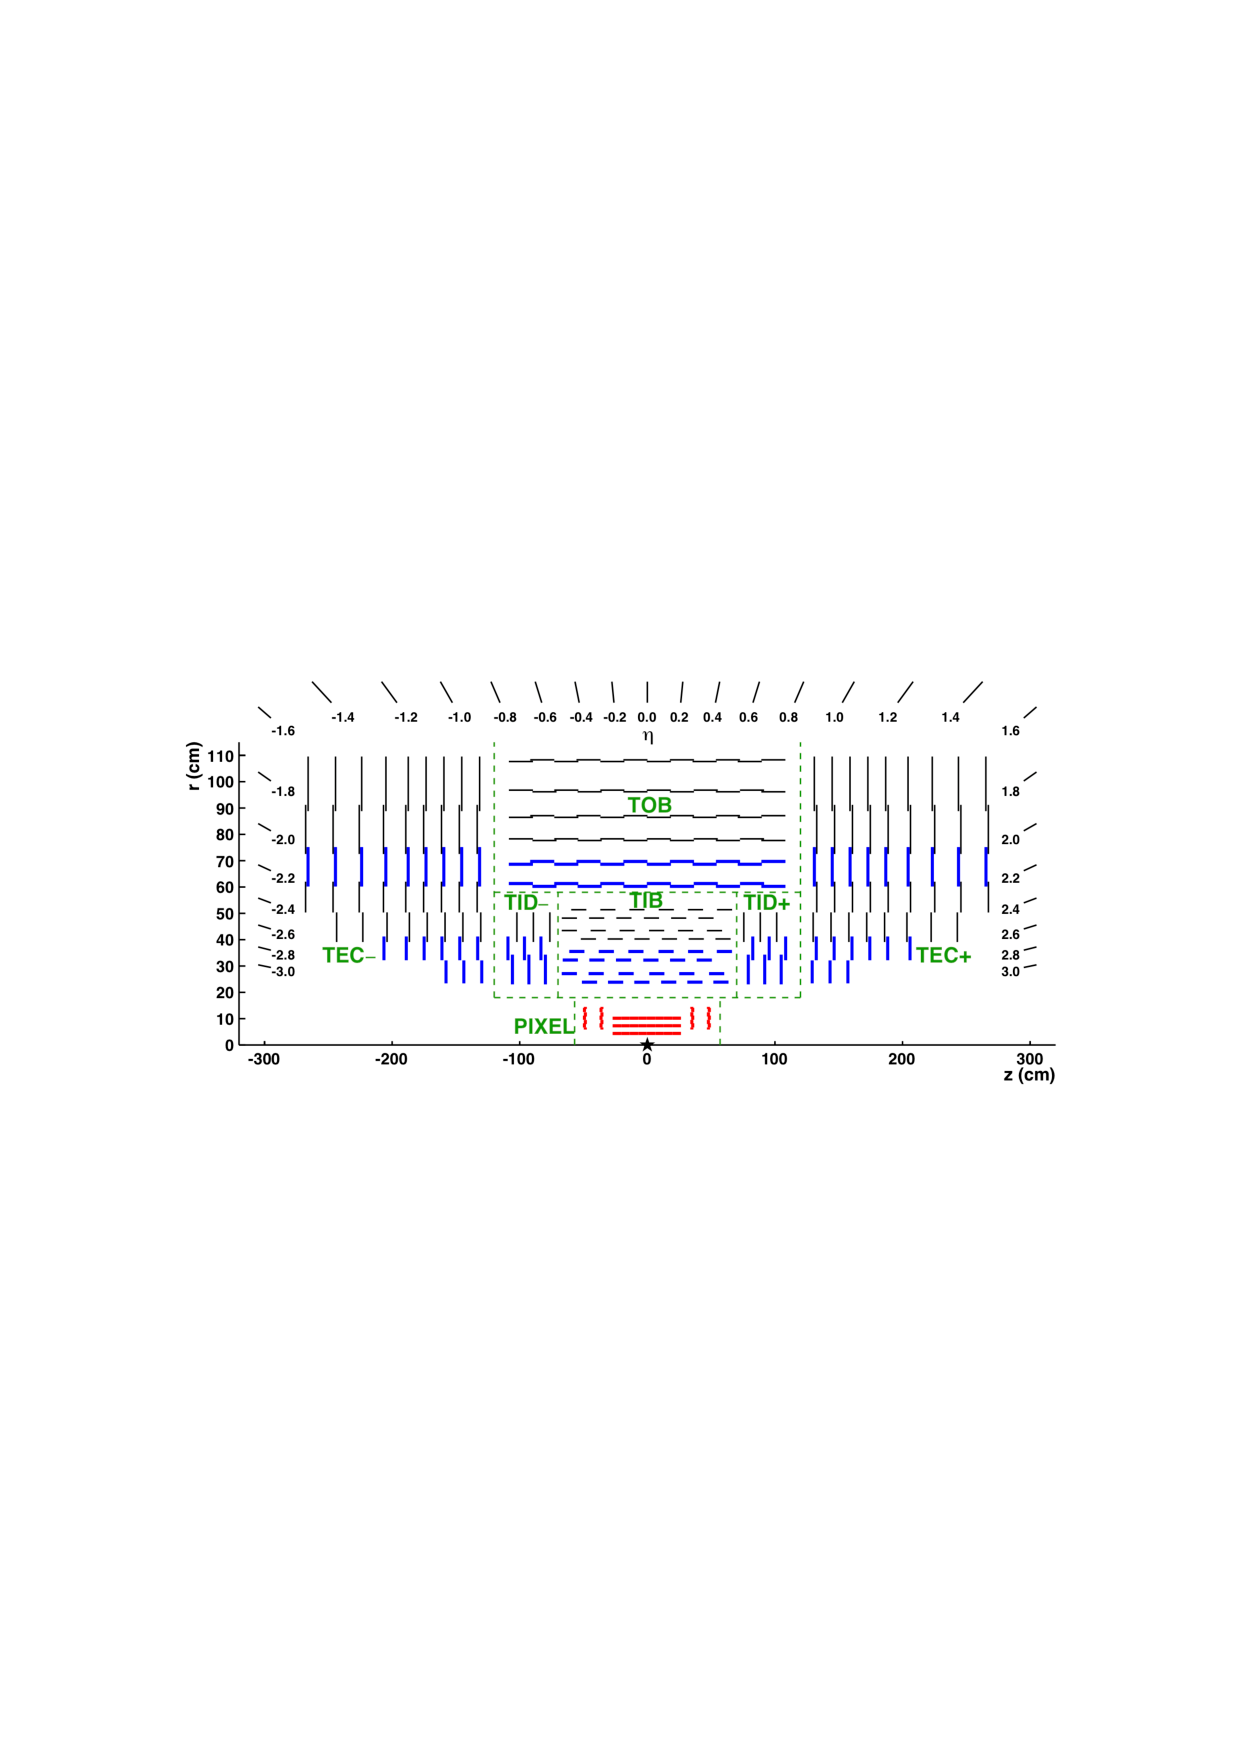
\includegraphics[width=\textwidth]{\PhDthesisdir/plots_and_images/from_CMS-TRK-17-001/CMS-TRK-17-001_Figure_001-a.pdf}
\caption[Schéma détaillé du trajectographe du détecteur CMS.]{Schéma détaillé du trajectographe du détecteur CMS dans le plan \plane{r}{z}~\cite{CMS-TRK-11-001,CMS-TRK-17-001}. Le trajectographe est symétrique par rapport à l'axe $r=0$, axe du faisceau. Le centre du trajectographe, correspondant approximativement au lieu des collisions, est indiqué par une étoile. Les différentes sous-parties du trajectographe sont délimitées par les pointillés verts. Les modules à fils donnant des signaux en deux dimensions sont indiqués en lignes noires fines et ceux donnant des signaux en trois dimensions en lignes bleues épaisses. Ces derniers sont en fait constitués de deux modules à fils dos à dos dont l'un est tourné de \ang{90}. Les modules à pixels, en rouge, permettent également d'obtenir des signaux à trois dimensions. Les légers décalages des modules leur permettent d'éviter tout angle mort dans la zone d'acceptance du détecteur.}
\label{fig-CMS-trk_detailed_scheme}
\end{figure}
\begin{figure}[p]
\centering
\subcaptionbox{Résolution pour des muons seuls et isolés.\label{subfig-chapter-LHC-section-CMS-subsec-tracker-pT-resolution-muons}}[.45\textwidth]
{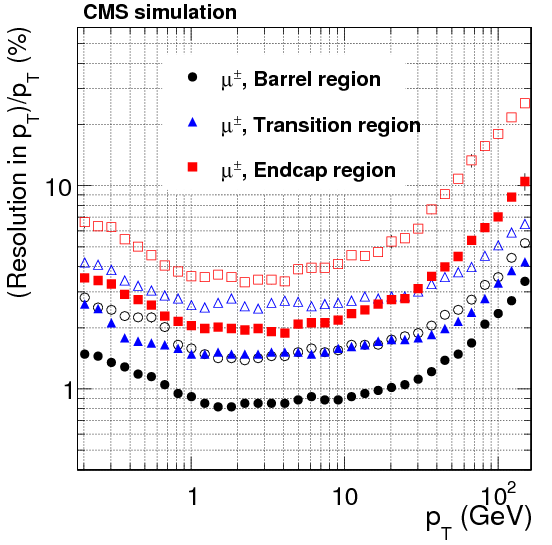
\includegraphics[width=.45\textwidth]{\PhDthesisdir/plots_and_images/from_CMS-TRK-11-001/figs_2011_trackPerformance_MC_SingleParticles_mu_resolutionPtVsPt.png}}
\hfill
\subcaptionbox{Résolution pour des particules chargées.\label{subfig-chapter-LHC-section-CMS-subsec-tracker-pT-resolution-charged_ptcs}}[.45\textwidth]
{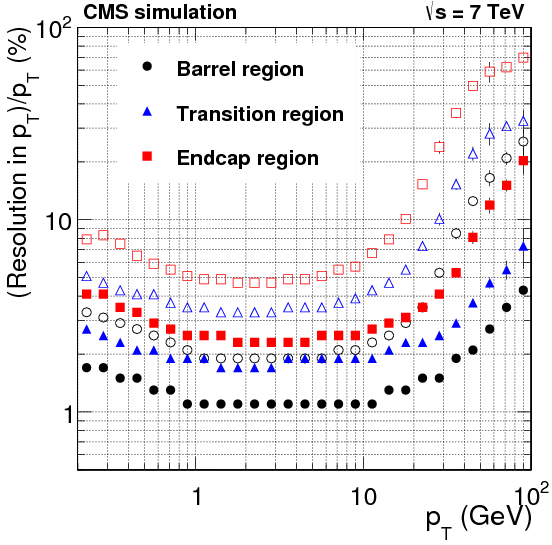
\includegraphics[width=.45\textwidth]{\PhDthesisdir/plots_and_images/from_CMS-TRK-11-001/figs_2011_trackPerformance_MC_ttbarHpWithPuSplitByEta_resolutionPtVsPt.png}}
\caption[Résolution en \pT\ du trajectographe.]{Résolution en \pT, en fonction de \pT, du trajectographe pour différentes particules~\cite{CMS-TRK-11-001}. Les symboles pleins correspondent à la demi-largeur à \SI{68}{\%} de la distribution, les symboles creux à \SI{90}{\%}.}
\label{fig-chapter-LHC-section-CMS-subsec-tracker-pT-resolution}
\end{figure}
Le trajectographe permet de reconstruire les trajectoires des particules chargées de pseudo-rapidité inférieure à \num{2.5}.
Ces particules laissent en effet des signaux de leur passage dans les différents modules du trajectographe.
Le trajectographe est ainsi essentiel à la reconstruction des vertex des événements du LHC.
\par Deux types de modules composent le trajectographe de CMS~\cite{cms_paper,CERN-LHCC-98-006,CMS-TDR-11,CMS-TRK-11-001,CMS-TRK-17-001}.
Dans sa partie la plus centrale, des modules à pixels de silicium sont utilisés.
Au début du Run II du LHC, trois couches de pixels sont présentes dans la partie barillet, à \num{4.4}, \num{7.3} et \SI{10.2}{\centi\meter} de rayon~\cite{cms_paper}, visibles en rouge sur la figure~\ref{fig-CMS-trk_detailed_scheme}.
Deux disques de pixels sont présents dans chacun des bouchons.
Les cellules des pixels ont une taille de $\num{100}\times\SI{150}{\micro\meter^2}$.
La résolution spatiale de cette partie du trajectographe est de l'ordre de \SI{10}{\micro\meter}~\cite{cms_paper} et permet d'obtenir une bonne reconstruction des vertex.
En mars 2017, cette partie du trajectographe est remplacée~\cite{cms_trk_upgrade_2017}.
Elle comporte alors quatre couches de pixels dans la partie barillet à \num{2.9}, \num{6.8}, \num{10.9} et \SI{16.0}{\centi\meter} de rayon.
Dans les bouchons, les disques sont également repensés afin d'obtenir quatre points de passage pour les traces telles que $\abs{\eta}\leq\num{2.5}$.
Une comparaison des trajectographes à pixels utilisés en 2016 (Phase-0) et à partir de 2017 (Phase-1) est illustrée sur la figure ~\ref{fig-chapter-LHC-section-CMS-subsec-tracker-2017-upgrade}.
Cette modification du détecteur permet d'améliorer la reconstruction des vertex ainsi que l'efficacité de l'identification de jets issus de quarks~\quarkb.
\begin{figure}[h]
\centering
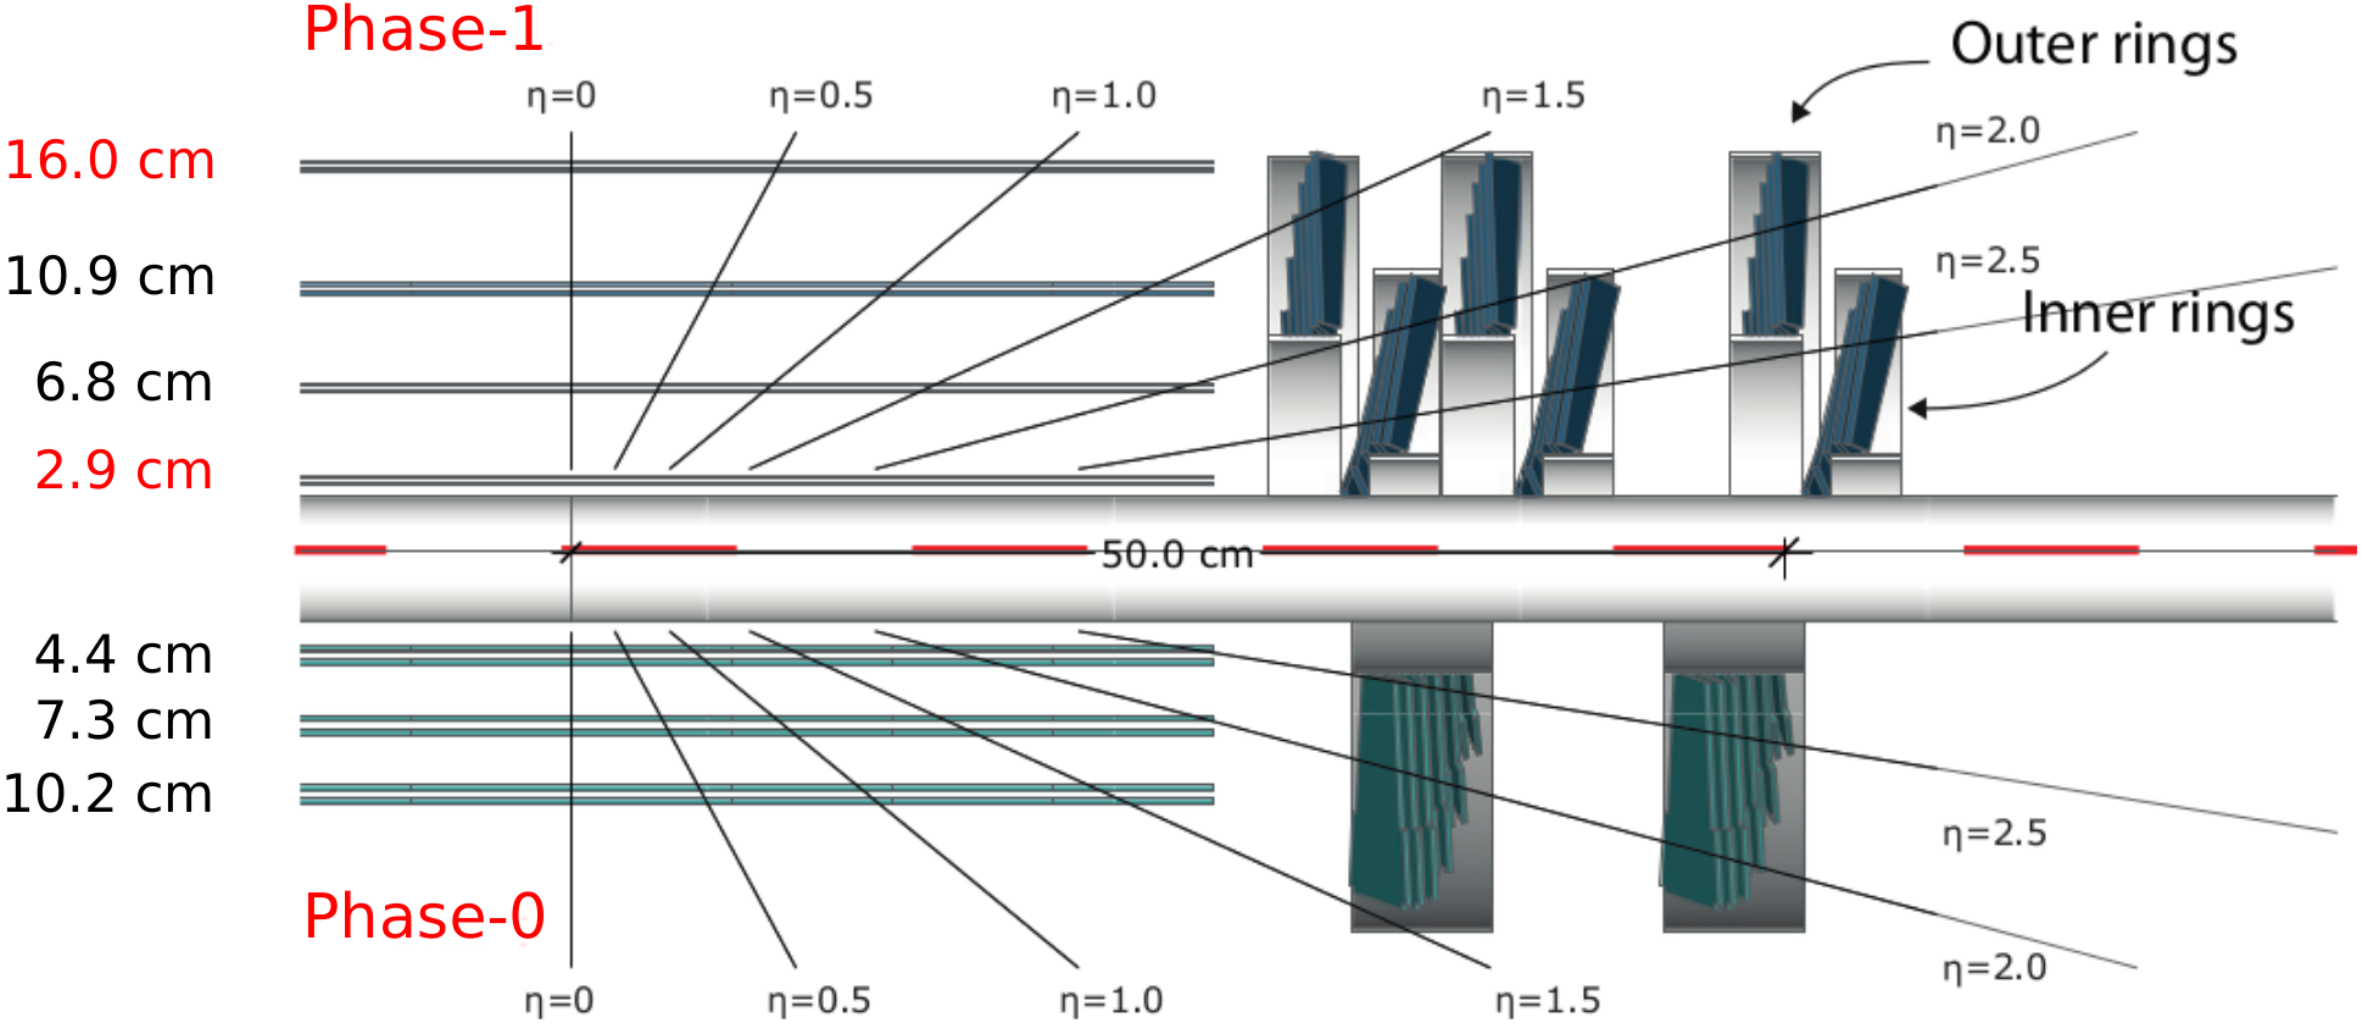
\includegraphics[width=0.8\linewidth]{\PhDthesisdir/plots_and_images/from_cms_trk_upgrade_2017/fig2.png}
\caption[Comparaison des trajectographes à pixels utilisés en 2016 (Phase-0) et à partir de 2017 (Phase-1).]{Comparaison des trajectographes à pixels utilisés en 2016 (Phase-0) et à partir de 2017 (Phase-1)~\cite{cms_trk_upgrade_2017}.}
\label{fig-chapter-LHC-section-CMS-subsec-tracker-2017-upgrade}
\end{figure}
\par De \num{20} à \SI{116}{\centi\meter} de rayon se trouve le trajectographe à fils, lui-même composé de trois sous-parties.
La première de ces sous-parties comporte le trajectographe interne du barillet (TIB, \emph{Tracker Inner Barrel}) de quatre couches et les trajectographes internes à disques (TID, \emph{Tracker Inner Disks}) de trois couches chacun.
Les fils de ces couches sont parallèles au faisceau dans le TIB et axiaux dans les TID.
Ils permettent d'obtenir une résolution de \SI{23}{\micro\meter} et \SI{35}{\micro\meter} respectivement~\cite{cms_paper}.
Le TIB et les TID sont entourés par le trajectographe externe du barillet (TOB, \emph{Tracker Outer Barrel}) de six couches.
Le TOB a une résolution de \SI{53}{\micro\meter} pour ses quatre premières couches et de \SI{35}{\micro\meter} ensuite~\cite{cms_paper}.
Enfin, les bouchons du trajectographe (TEC, \emph{Tracker EndCaps}) se situent aux extrémités du dispositif.
\par Les trajectoires des particules chargées sont alors reconstruites par interpolation entre les différents points de passage dans le trajectographe compatibles avec la trajectoire d'une particule.
À partir de ces trajectoires, il est possible de déterminer l'impulsion transverse des particules à l'aide de l'équation~\eqref{eq-chapter-LHC-section-CMS-subsec-solenoide-rayon_courbure}.
Les résolutions obtenues sur les impulsions transverses des muons et de particules chargées à l'aide du trajectographe sont présentées sur la figure~\ref{fig-chapter-LHC-section-CMS-subsec-tracker-pT-resolution}.
